\documentclass[10pt,a4paper]{article}
\usepackage[utf8]{inputenc}
\usepackage[german]{babel}
\usepackage{mathrsfs}
\usepackage{amsmath}
\usepackage{amsfonts}
\usepackage{amssymb}
\usepackage{amsthm}
\usepackage[left=2cm,right=2cm,top=2cm,bottom=2cm]{geometry}
\usepackage{tikz}
\usetikzlibrary{automata,positioning}
\usepackage{graphicx}

\begin{document}

\section{Aufgabe 1.1}

\subsection{Teil a}

\subsubsection{(i)}

\begin{equation}
  F \Rightarrow \lnot B
\end{equation}

\subsubsection{(ii)}

\begin{equation}
  \lnot F \Rightarrow (B \land D)
\end{equation}

\subsubsection{(iii)}

\begin{equation}
  (\lnot B \lor D) \Rightarrow (F \land M)
\end{equation}

\subsubsection{(iv)}

\begin{equation}
  M \Rightarrow G
\end{equation}

\subsection{Teil b}

\subsubsection{(i)}

\begin{equation}
  (F \Rightarrow \lnot B) \Leftrightarrow (\lnot F \lor \lnot B)
\end{equation}

\subsubsection{(ii)}

\begin{equation}
  (\lnot F \Rightarrow (B \land D)) \Leftrightarrow (F \lor (B \land D)) \Leftrightarrow ((F \lor B) \land (F \lor D))
\end{equation}

\subsubsection{(iii)}

\begin{align*}
  ((\lnot B \lor D) \Rightarrow (F \land M)) \Leftrightarrow & (\lnot(\lnot B \lor D) \lor (F \land M))\\
  \Leftrightarrow & ((B \land \lnot D) \lor (F \land M))\\
  \Leftrightarrow & (((B \lor (F \land M)) \land (\lnot D \lor (F \land M)))\\
  \Leftrightarrow & ((B \lor F) \land (B \lor M) \land (\lnot D \lor F) \land (\lnot D \lor M))\\
\end{align*}

\subsubsection{(iv)}

\begin{equation}
  (M \Rightarrow G) \Leftrightarrow (\lnot M \lor G)
\end{equation}

\subsection{Teil c}

Annahme $\lnot G$.
Die Klauselmenge ist
\begin{equation}
  \{ \lnot F, \lnot B \}, \{ F, B \}, \{ F, D \}, \{ B, F \}, \{ B, M \}, \{ \lnot D, F \}, \{ \lnot D, M \}, \{ \lnot M, G \}, \{ \lnot G \}
\end{equation}
Verknüpfung der letzten beiden Klauseln ergibt
\begin{equation}
  \{ \lnot M \}
\end{equation}
Verknüpfung von $\{ \lnot F, \lnot B \}$ und $\{ F, D \}$ ergibt
\begin{equation}
  \{ \lnot B, D \}
\end{equation}
Verknüpfung von $\{ \lnot B, D \}$ und $\{ B, M \}$ ergibt
\begin{equation}
  \{ D, M \}
\end{equation}
Verknüpfung von $\{ D, M \}$ und $\{ \lnot D, M \}$ ergibt
\begin{equation}
  \{ M \}
\end{equation}
Verknüpfung von $\{ M \}$ und $\{ \lnot M \}$ ergibt
\begin{equation}
  \{ \}
\end{equation}
Somit ist die Annahme falsch und der Yeti muss ein PR-Gag sein.

\section{Aufgabe 1.2}

\subsection{Teil a}

\subsubsection{(i)}

\begin{align*}
  \hat{\delta}(\{z_{0}\}, cbcbaba) & = \hat{\delta}(\{ z_{0} \}, bcbaba)\\
  & = \hat{\delta}(\{ z_{0}, z_{3} \}, cbaba)\\
  & = \hat{\delta}(\{ z_{0} \}, baba)\\
  & = \hat{\delta}(\{ z_{0}, z_{3} \}, aba)\\
  & = \hat{\delta}(\{ z_{1}, z_{3} \}, ba)\\
  & = \hat{\delta}(\{ z_{2}, z_{3} \}, a)\\
  & = \{ z_{2}, z_{3} \}
\end{align*}
\begin{equation}
  \{ z_{2}, z_{3} \} \cap \{ z_{1}, z_{3} \} \ne \emptyset
\end{equation}
Man erreicht also einen Finalzustand und somit ist das Wort enthalten.

\subsubsection{(ii)}

\begin{align*}
  &
  \begin{cases}
    z_{0} & = bz_{0} + cz_{0} + az_{1} + bz_{3}\\
    z_{1} & = bz_{2} + bz_{3}\\
    z_{2} & = cz_{1}\\
    z_{3} & = az_{3}
  \end{cases}
  \\\Leftrightarrow &
  \begin{cases}
    z_{0} & = bz_{0} + cz_{0} + az_{1} + bz_{3}\\
    z_{1} & = bz_{2} + bz_{3}\\
    z_{2} & = cz_{1}\\
    z_{3} & = a^{*}
  \end{cases}
  \\\Leftrightarrow &
  \begin{cases}
    z_{0} & = (b + c)z_{0} + az_{1} + ba^{*}\\
    z_{1} & = bz_{2} + ba^{*}\\
    z_{2} & = cz_{1}\\
    z_{3} & = a^{*}
  \end{cases}
  \\\Leftrightarrow &
  \begin{cases}
    z_{0} & = (b + c)^{*}(az_{1} + ba^{*})\\
    z_{1} & = bcz_{1} + ba^{*}\\
    z_{2} & = cz_{1}\\
    z_{3} & = a^{*}
  \end{cases}
  \\\Leftrightarrow &
  \begin{cases}
    z_{0} & = (b + c)^{*}(az_{1} + ba^{*})\\
    z_{1} & = (bc)^{*}ba^{*}\\
    z_{2} & = cz_{1}\\
    z_{3} & = a^{*}
  \end{cases}
  \\\Leftrightarrow &
  \begin{cases}
    z_{0} & = (b + c)^{*}(a(bc)^{*}ba^{*} + ba^{*})\\
    z_{1} & = (bc)^{*}ba^{*}\\
    z_{2} & = cz_{1}\\
    z_{3} & = a^{*}
  \end{cases}
\end{align*}

\begin{equation}
  \gamma = (b + c)^{*}(a(bc)^{*}ba^{*} + ba^{*})
\end{equation}

\subsubsection{(iii)}

Definiere $N = (\{ a, b, c \}, \{  \}, \delta_{N}, \{ z_{0} \}, \{  \})$.
Die Übergänge $\delta_{N}$ sind gegeben durch
\\
\begin{tikzpicture}[node distance=3cm, on grid, auto]
  \node[state,initial] (z0) {$\{ z_{0} \}$};
  \node[state,accepting] (z1) [right=of z0] {$\{ z_{1} \}$};
  \node[state,accepting] (z3) [above=of z1] {$\{ z_{3} \}$};
  \node[state,accepting] (z0z3) [below left=of z0] {$\{ z_{0}z_{3} \}$};
  \node[state] (x) [right=of z1] {$\{  \}$};
  \node[state,accepting] (z1z3) [above=of z0] {$\{ z_{1}z_{3} \}$};
  \node[state,accepting] (z2z3) [below left=of z1] {$\{ z_{2}z_{3} \}$};
  \path[->]
  (z0) edge node {a} (z1)
  (z0) edge [bend left] node {b} (z0z3)
  (z0) edge [loop above] node {c} (z0)
  (z1) edge [bend right] node {a} (x)
  (z1) edge [bend left] node {b} (z2z3)
  (z1) edge node {c} (x)
  (z3) edge [loop above] node {a} (z3)
  (z3) edge [bend left] node {b} (x)
  (z3) edge node {c} (x)
  (z0z3) edge [bend left] node {a} (z1z3)
  (z0z3) edge [loop below] node {b} (z0z3)
  (z0z3) edge node {c} (z0)
  (z1z3) edge node {a} (z3)
  (z1z3) edge node {b} (z2z3)
  (z1z3) edge node {c} (x)
  (z2z3) edge node {a} (z3)
  (z2z3) edge node {b} (x)
  (z2z3) edge node {c} (z1)
  ;
\end{tikzpicture}

\subsection{Teil b}

\begin{tabular}{c|c|c|c|c|c}
  & $z_{0}$ & $z_{1}$ & $z_{2}$ & $z_{3}$ & $z_{4}$\\\hline
  $z_{4}$ & x & x & x &   & -\\\hline
  $z_{3}$ & x & x & x & - & -\\\hline
  $z_{2}$ & x &   & - & - & -\\\hline
  $z_{1}$ & x & - & - & - & -\\\hline
  $z_{0}$ & - & - & - & - & -
\end{tabular}
\\
Man kann also die Zustände $z_{1}, z_{2}$ und $z_{3}, z_{4}$ verschmelzen.
Der Minimalautomat ist dann
\\
\begin{tikzpicture}[node distance=3cm, on grid, auto]
  \node[state,initial] (z0) {$z_{0}$};
  \node[state,accepting] (z1z2) [right=of z0] {$z_{1}z_{2}$};
  \node[state] (z3z4) [right=of z1z2] {$z_{3}z_{4}$};
  \path[->]
  (z0) edge [bend left] node {a} (z1z2)
  (z0) edge [bend right] node {b} (z1z2)
  (z1z2) edge [bend left] node {b} (z3z4)
  (z3z4) edge [loop right] node {a} (z3z4)
  (z3z4) edge [bend left] node {c} (z1z2)
  ;
\end{tikzpicture}

\section{Aufgabe 1.3}

\subsection{Teil a}

\begin{proof}
  Sei $n$ die untere Grenze aus dem Pumpinglemma.
  Man betrachte $a^{n}b^{j}$ mit $n + j \ge n$ und $n + j$ prim und so, dass der Abstand zwischen $n + j$ und der nächsten Primzahl größer als $n$ ist.
  Ein solches $j$ existiert nach dem Satz von Euklid und weil Primzahlen für große Zahlen beliebig selten werden.
  Sei $uvw$ eine aufpumpbare Zerlegung mit $|v| \ge 1$ und $|uv| \le n$.
  Dann ist $v = a^{i}$ für ein $i \in \mathbb{N}$, weil $|uv| \le n$ und $a^{n}$ ein Präfix von $uvw$ ist.
  Nach der Vorraussetzung ist $uv^{2}w \not\in L$, weil die nächste Primzahl weiter als $n$ von $n + j$ entfernt ist.
\end{proof}

\subsection{Teil b}

$L_{1}$ ist nicht regülär.
$L_{1}$ ist die Sprache, wo $i$ $a$s von $i$ $b$s gefolgt sind und $i$ eine echt positive gerade Zahl ist.
Es gibt also unendlich viele Äquivalenzklassen, nämlich mindestens eine für jedes $a^{2i}$ mit $i \in \mathbb{N}$, weil
\begin{equation}
  (a^{2j} \equiv a^{2i}) \Rightarrow (a^{2i}b^{2j} \in L_{1}) \Rightarrow 2i = 2j \Rightarrow i = j
\end{equation}
Da das letzte aber für alle Paare $(i, j) \in \mathbb{N}^{2}$ mit $i \ne j$ nicht wahr ist, kann auch schon der erste nicht wahr sein und $a^{2i}$ und $a^{2j}$ müssen in unterschiedlichen Äquivalenzklassen sein.

Die Äquivalenzklassen von $L_{2}$ sind
\begin{align*}
  [a] & = \{ a, aaa, aaaaa, \dots \} = \{ \textit{Worte, die drin sind, wenn man $a^{i}b^{j}$ mit $i + j = 2k + 1$ für $k \ge 1$ anhängt} \}\\
  [aa] & = \{ \lambda, aa, aaaa, aaaaaa, \dots \} = \{ \textit{Worte, die drin sind, wenn man ein Wort aus $L_{2}$ anhängt} \}\\
  [b] & = \{ b, bbb, abb, aab, \dots \} = \{ \textit{Worte, die drin sind, wenn man eine ungerade Anzahl von $b$s anhängt} \}\\
  [bb] & = \{ bb, bbbb, aabb, aaaaaabb, \dots \} = \{ \textit{Worte, die drin sind, wenn man eine gerade Anzahl von $b$s anhängt} \}\\
  [ba] & = \{ ba, baaaabbba, baba, bbbbba, \dots \} = \{ \textit{Worte, die nie drin sind} \}
\end{align*}
Dies ist eine Zerlegung von $\Sigma^{*}$, also ist $L_{2}$ regulär.

Also ist $L_{2}$ regulär.
Worte sind beliebig viele $a$s gefolgt von beliebig vielen $b$s mit der Einschränkung, dass die gesamte Wortlänge gerade ist.
Es sind also entweder eine gerade Anzahl von $a$s gefolgt von einer gerade Anzahl von $b$s oder eine ungerade Anzahl von $a$s gefolgt von einer weiteren ungeraden Anzahl von $b$s.
Ein DFA, der dies akzeptiert ist definiert durch $N = (\{ a, b \}, \{  \}, \delta, z_{0}, \{  \})$, wobei die Übergänge $\delta$ wie folgt aussehen.
\\
\begin{tikzpicture}[node distance=3cm, on grid, auto]
  \node[state,initial,accepting] (z0) {$z_{0}$};
  \node[state] (z1) [above=of z0] {$z_{1}$};
  \node[state] (z2) [right=of z0] {$z_{2}$};
  \node[state,accepting] (z3) [above=of z2] {$z_{3}$};
  \node[state] (z4) [above right=of z2] {$z_{4}$};
  \path[->]
  (z0) edge [bend right] node {a} (z1)
  (z0) edge node {b} (z2)
  (z1) edge [bend right] node {a} (z0)
  (z1) edge node {b} (z3)
  (z2) edge node {a} (z4)
  (z2) edge [bend right] node {b} (z3)
  (z3) edge node {a} (z4)
  (z3) edge [bend right] node {b} (z2)
  (z4) edge [loop above] node {a} (z4)
  (z4) edge [loop below] node {b} (z4)
  ;
\end{tikzpicture}

\section{Aufgabe 1.4}

\subsection{Teil a}

Die Grammatik enthält keine $\lambda$-Regeln.
Also muss zuerst die eine einfache Regel eliminiert werden.
Dann ist $P$ gegeben durch
\begin{equation}
  \{ S \rightarrow 0BCBA, C \rightarrow 0BCBA | 0, A \rightarrow 0, B \rightarrow 1 \}
\end{equation}
Die Produktionen der Chomsky-Normalform $G' = (\{ 0, 1 \}, \{ S, S', S'', S''', A, B, C \})$ sind dann
\begin{equation}
  \{ S \rightarrow AS', S' \rightarrow BS'', S'' \rightarrow CS''', S''' \rightarrow BA, C \rightarrow AS' | 0, A \rightarrow 0, B \rightarrow 1 \}
\end{equation}

\subsection{Teil b}

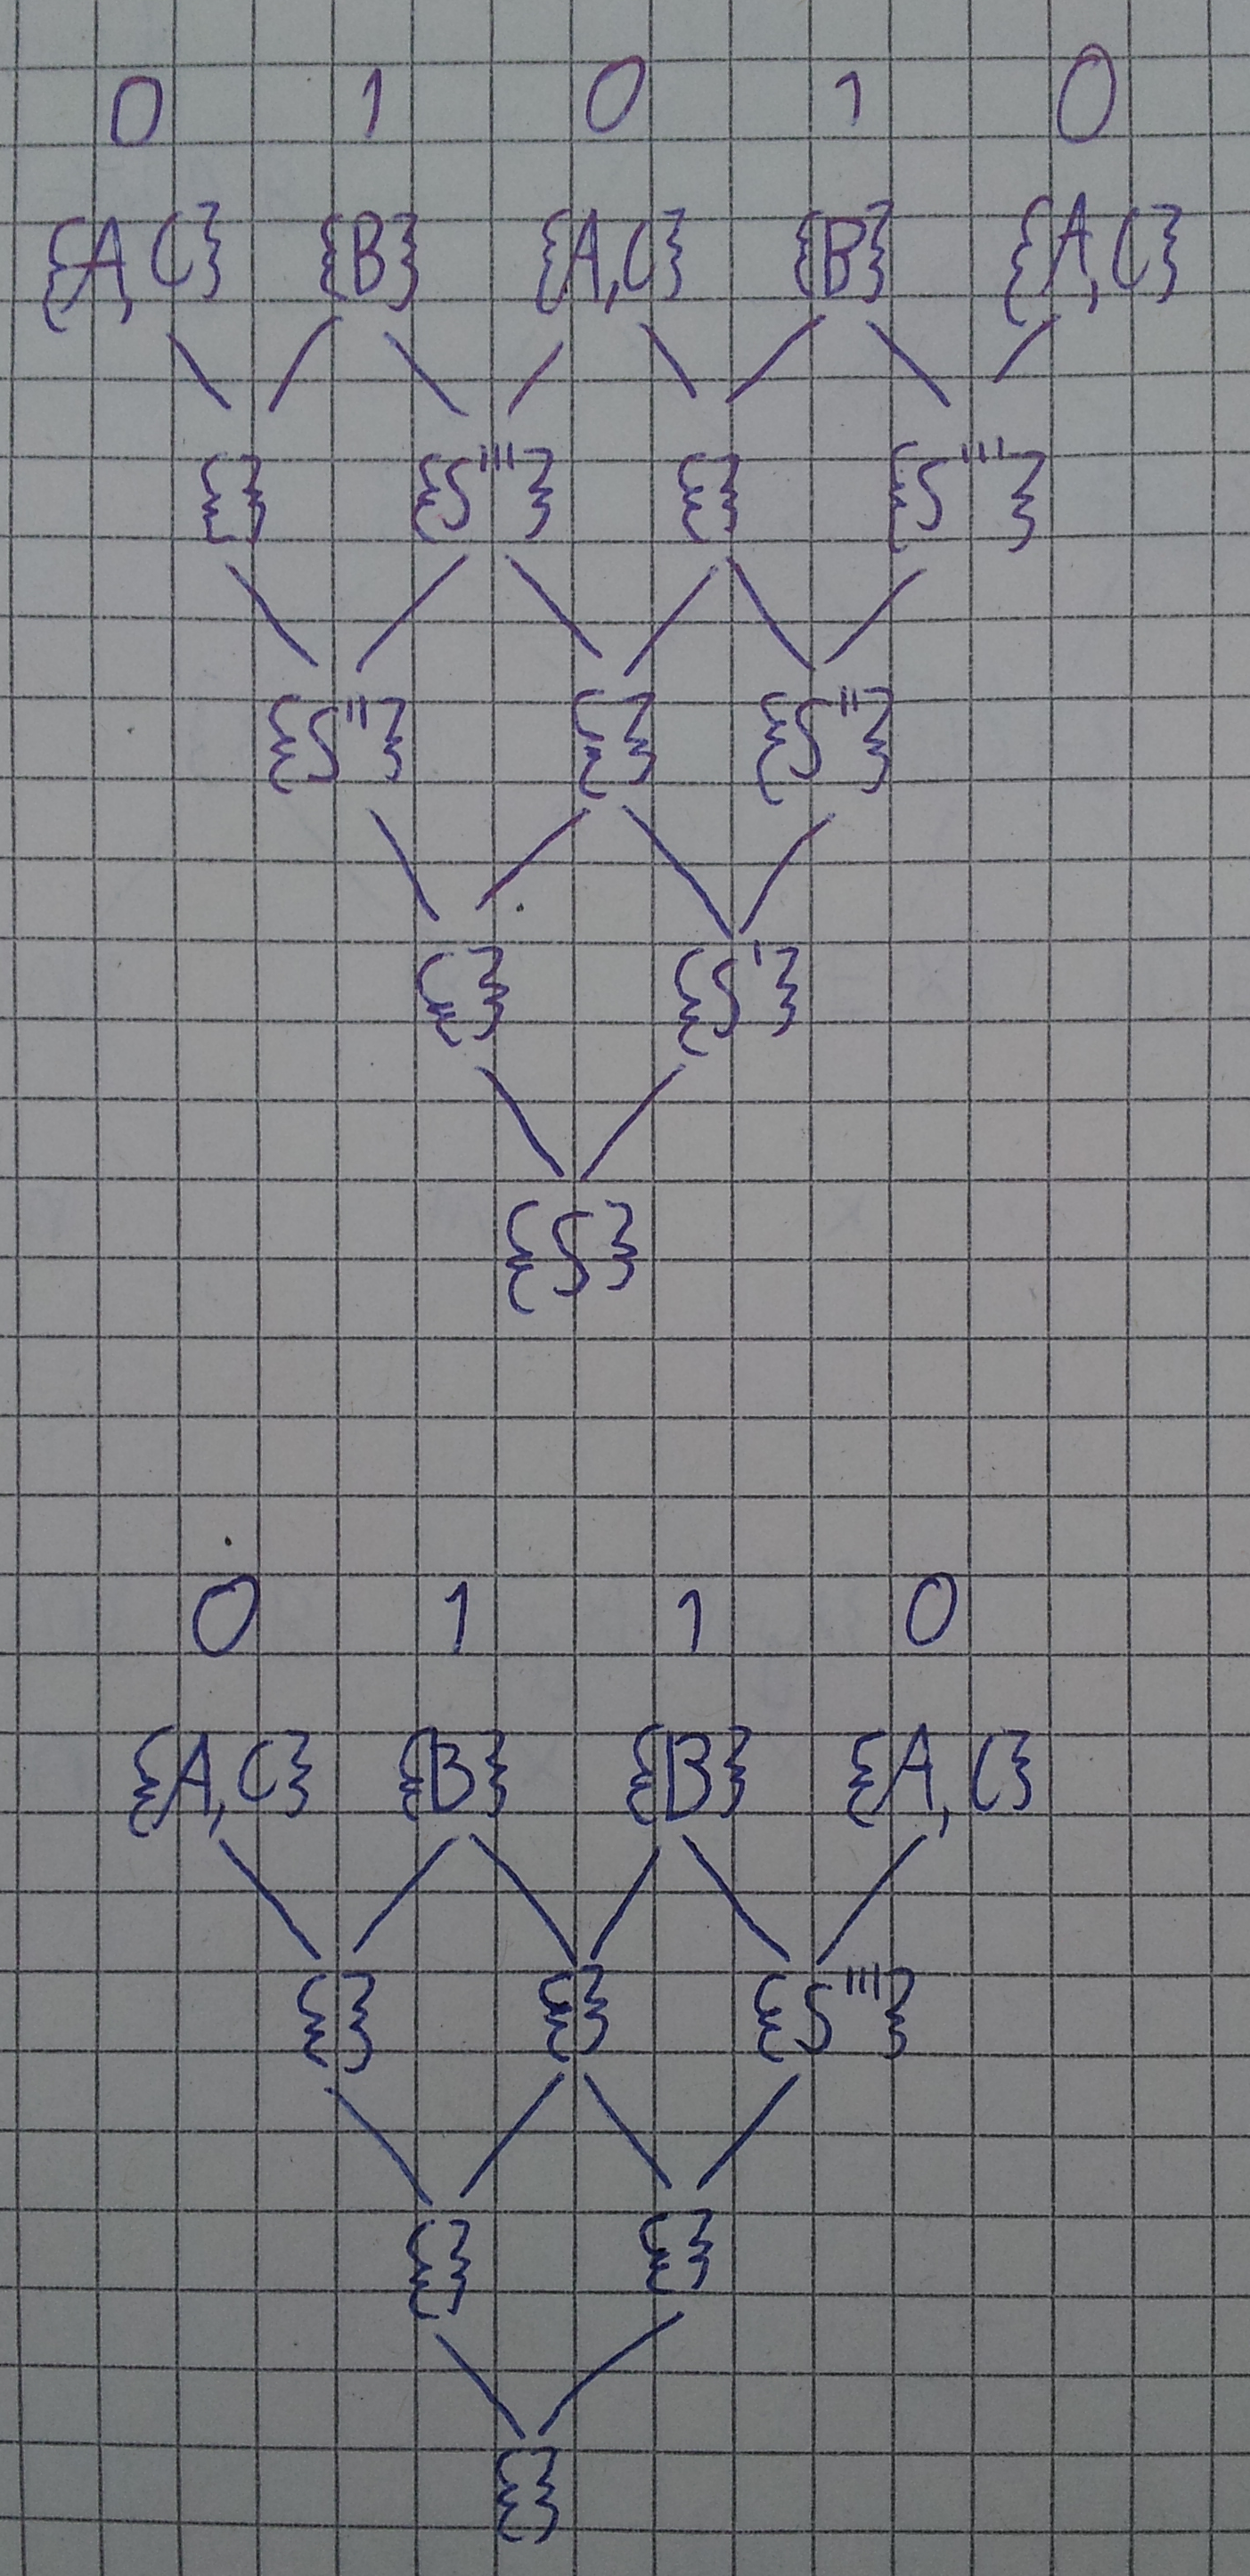
\includegraphics[width=300pt]{7_4_b.png}

$w_{1}$ ist also drin, aber nicht $w_{2}$.

\subsection{Teil c}

\begin{equation}
  \Psi(L(G)) = \{ (3, 2) + b \cdot (2, 2) \mid b \in \mathbb{N}_{0} \}
\end{equation}
Nach dem Algorithmus ist
\begin{equation}
  \gamma = 0^{3}1^{2}(0^{2}1^{2})^{*}
\end{equation}

\subsection{Teil d}

\begin{equation}
  L(G) = \{ (01)^{i}0(10)^{i} \mid i \in \mathbb{N}, i \ge 1 \}
\end{equation}

\section{Aufgabe 1.5}

Definiere den nicht-deterministischen Kellerautomaten $N$ als
\begin{equation}
  (\{ a, b \}, \{ A, # \}, \{ z_{0}, z_{1} \}, \delta, z_{0}, \#)
\end{equation}
mit der Überführungsfunktion $\delta$ definiert durch
\begin{align*}
  z_{0}a\# & \rightarrow z_{0}A\#\\
  z_{0}aA & \rightarrow z_{0}AA\\
  z_{0}b\# & \rightarrow z_{1}\#\\
  z_{0}bA & \rightarrow z_{0}\\
  z_{0}\lambda\# & \rightarrow z_{0}\\
  z_{1}a\# & \rightarrow z_{1}\#\\
\end{align*}
Wenn man einmal in Zustand $z_{1}$ ist, wird also niemals der Stapel leer werden.
Das Lesen eines $a$s, legt ein $A$ auf den Stapel, was es ermöglicht, später ein $b$ zu lesen, ohne in den Zustand $z_{1}$ zu wechseln.
Wenn man jedoch ein $b$ liest, ohne vorher ein entsprechendes $a$ gelesen zu haben, kann das Wort die Vorraussetzung nicht mehr erfüllen und man wechselt in den Zustand $z_{1}$.
$N$ akzeptiert also genau die Wörter, deren Präfixe höchstens so viele $b$s wie $a$s enthalten.

\end{document}